\documentclass[a4paper,14pt]{extarticle}
%\usepackage{cmap}					% поиск в PDF
%\usepackage{pscyr}
%%% Работа с русским языком
\usepackage[english]{babel}   %% загружает пакет многоязыковой вёрстки
\usepackage{fontspec}      %% подготавливает загрузку шрифтов Open Type, True Type и др.
\defaultfontfeatures{Ligatures={TeX},Renderer=Basic}  %% свойства шрифтов по умолчанию
\setmainfont[Ligatures={TeX,Historic}]{Liberation Serif} %% задаёт основной шрифт документа
\setsansfont{Liberation Sans}                    %% задаёт шрифт без засечек
\setmonofont{Liberation Mono}
\usepackage{indentfirst}
\frenchspacing
%\usepackage[T2A]{fontenc}			% кодировка
%\usepackage[utf8]{inputenc}			% кодировка исходного текста
%\usepackage[english, russian]{babel}	% локализация и переносы
%\usepackage{mathtools}              % математика
\usepackage{hyperref}               % гиперссылки
\usepackage{amsmath,amsfonts,amssymb,amsthm,mathtools} % AMS
%\usepackage{icomma} % "Умная" запятая: $0,2$ --- число, $0, 2$ --- перечисление
%%% Работа с картинками
\usepackage{graphicx}  % Для вставки рисунков
%%% Картинки
\usepackage{tikz} % Работа с графикой
\usepackage{pgfplots}
\usepackage{pgfplotstable}
\usepackage{multicol}
\usepackage{amsfonts}
\usepackage{color}
\usepackage{enumitem}
\usepackage{setspace} % Интерлиньяж
\usepackage{listings}
\usepackage[title,titletoc]{appendix}
%\onehalfspacing % Интерлиньяж 1.5
\linespread{1}
\usepackage[style=gost-numeric,maxcitenames=2,backend=biber,sorting=none]{biblatex}

\addbibresource{dl.bib}

\newcommand{\empline}{\mbox{}\newline} % пустая строка

%\newcommand{\append}[1]{
%    \clearpage
%    \stepcounter{section}
%    \begin{flushright}%
%        \textbf{Приложение \Asbuk{section}}
%    \end{flushright}
%    \begin{center}\textbf{{#1}}\end{center}
%    \empline
%    \addcontentsline{toc}{section}{\Asbuk{section}\hspace{0.6em}~#1}}

\pgfplotsset{compat=1.11}
\usepackage{listings}
\usepackage{caption}
\usepackage{pdfpages}
\captionsetup[figure]{labelfont=bf}
\captionsetup[table]{labelfont=bf}
\usepackage{geometry} % Меняем поля страницы
\geometry{left=2cm}% левое поле
\geometry{right=1.5cm}% правое поле
\geometry{top=1cm}% верхнее поле
\geometry{bottom=2cm}% нижнее поле
\usepackage{float}
\usepackage[labelformat=simple]{subcaption}
\usepackage{booktabs}
\newcommand{\todo}[1]{
    (\textbf{\underline{{\colorbox{yellow}{TODO: }}}}\textit{\color{cyan}{#1}})
}
\usepackage{graphicx}
\DeclareMathOperator*{\argmin}{arg\,min}
\DeclareMathOperator{\E}{\mathbb{E}}
\begin{document}

\title{
\vspace{5cm}
	"Opening the black box of Deep Neural Networks via Information" by Schwarz-Ziv and Tishby
	\newline
	\Large Report for "Graphical Models and Statistical Inference" course  at Skoltech}
\author{Bogdan Kirillov}

\maketitle

\numberwithin{equation}{section}
\numberwithin{figure}{section}
\numberwithin{table}{section}

\newpage

\tableofcontents

\newpage

\section{Introduction}
\subsection{Short description of the problem}
\paragraph{}
Recenlty attention of world's A.I. scientists is centered on Deep Neural Networks. The reason why is DNNs performance which is close to\cite{esteva2017dermatologist} and sometimes above human levels. DNNs can solve a lot of problems that were considered human-complete before with results that even surpasses human's abilities\cite{lu2015surpassing}.
\paragraph{}
This power comes with the following critical issues: 
\subparagraph{Lack of theory}
Currently there is no real theory behind why do the DNNs work. DNNs are large non-linear dynamical systems, among the largest that humanity ever encountered. The complexity of DNNs stops attempts to unravel their inner mechanics by classical mathematical methods.
\subparagraph{Black box}
Understanding why did the network put that particular label for this particular example is also very challenging. The DNNs are used today as black-box model without reliable possibility of interpretation. Graying this black box is an area of active research now\cite{liu2017towards}.
\paragraph{}
Because of those facts the field has limitations in its applicability: one wouldn't really use an algorithm that one doesn't understand completely (and actually nobody does), especially in serious settings when human lives depend on the model, e.g. in medicine, disaster mitigation, criminal investigations etc. 
\paragraph{}
The paper we are talking about\cite{shwartz2017opening} is written to shed light on the first issue. It provides an attempt to describe DNN's \textit{modus operandi} theoretically by applying modern methods of pure mathematics.
\subsection{Key points of the paper by Schwarz-Ziv and Tishby}
\paragraph{}
The paper of interest\cite{shwartz2017opening} can be roughly summarized to the following list of key points:
\begin{itemize}
		\item Most of the training time is spent on compression of the input to efficient representation rather than on fitting to labels;
		\item The compression begins when the training errors shrink and the SGD epochs go into random diffusion, constrained by the training error value;
		\item The converged layers lie very close to the theoretical bound, and the maps from the input to any hidden layer and from this hidden layer to the output satisfy the IB self-consistent equations. This mechanism is absent in one layer networks;
		\item The output of a neuron in hidden layer is irrelevant to the prediction of label \textit{per se}. Only the layered structure counts;
		\item Adding more hidden layers reduces training time;
		\item Hidden layers are expected to converge to critical points for phase transition of Informational Bottleneck curve.
	\end{itemize}
\subsection{Structure of this report}
\paragraph{}
This report is structured as follows:
\begin{enumerate}
	\item The first part of the report is intended to describe the contributions of Schwarz-Ziv and Tishby I have considered significant; \begin{itemize}
		\item Section "Information theory of Deep Learning" describes how the authors state the ways to apply classical information-theoretic approaches for the field of Deep Learning;
		\item Section "Network behavior on Information Plane" speaks about what Information Plane is and why authors consider it significant for the problem of Deep Neural Network Interpretation;
		\item Section "Hidden layers" concentrates on explanation of hidden layers \textit{modus operandi} provided by Schwarz-Ziv and Tishby;
	\end{itemize}
	\item The second part is left for description of my numerical experiments intended to reproduce some of the paper's plots and computations on a different setting; \begin{itemize}
		\item Section "Numerical experiments setup" describes differences of my setup compared to Schwarz-Ziv and Tishby's;
		\item Section "Results of numerical experiments" shows how my results differ from and how converge to Schwarz-Ziv and Tishby's, also here I speculate about the reason and meaning of the differences.
	\end{itemize}
	\item The third part roughly reviews current applications of the paper and foreshadows possible future extensions of the field.
\end{enumerate}

\section{Information theory of Deep Learning}
\paragraph{}
Main reason to do supervised learning is to get some representation of input data that aids prediction of a label (doesn't matter whether it is integer as in Classification or real as in Regression) not only on the training set but also in general case on data previously not seen by the model. One would want to be able to learn such representation from experimental data given the joint distribution of input data and labels is unknown. 
\paragraph{}
In their previous work\cite{tishby2015deep}, the authors suggested that DNNs form a Markov chain of such representations. They take form of network's hidden layer. Their first important insight is to consider output of a layer as single multidimensional random variable with its own decoder ($P(Y|T)$) and encoder ($P(T|X)$) distributions (as shown on figure below).
\begin{figure}[!h]
	\centering
	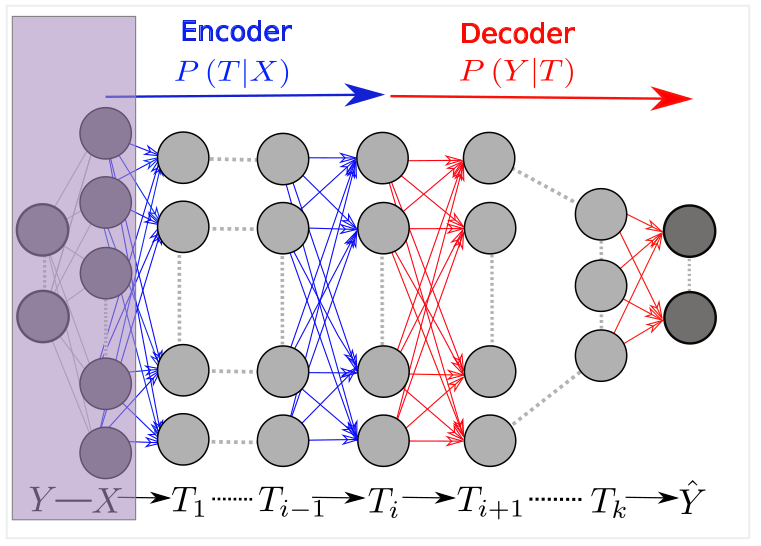
\includegraphics[width=\textwidth]{../presentation/MarkovChain.png}
	\caption{Markov chain of successive representations. T - representation, X - input, Y - label.}
\end{figure}
\paragraph{}
Before I define an Information Plane as the authors do, important things should be stated about the measures they use.
\paragraph{}
Their work is built around the Mutual Information:
\begin{equation}
	I(Input;Label) = D_{KL}[p(i,l)||p(i)p(l)] = \sum_{l \in Label; i \in Input} p(i,l) log\frac{p(i,l)}{p(i)p(l)}
\end{equation}
This formula basically means the following: if one receives two messages, the amount of redundant information one gets is equal to Kullback-Leibler divergency between their joint distribution and a multiplication of their distributions. By "redundant" I mean the information both messages share.
\paragraph{}
MI has two important properties (according to authors):
\subparagraph{Invariance to invertible transformations} 
\begin{equation}
	\forall \phi, \gamma: \exists \phi^{-1}, \gamma^{-1} \Rightarrow I(A;B) = I(\phi(A);\gamma(B))
\end{equation}
Mutual information remains unchanged if we apply to data some transformation that has an inverse.
\subparagraph{Data-Processing Inequality}
\begin{equation}
	\forall X,Y,Z: (X \rightarrow Y \rightarrow Z) \Rightarrow I(X;Y) \geq I(X;Z)
\end{equation}
where $A\rightarrow B ... \rightarrow Z$ - Markov chain, $X,Y,Z$ - random variable.\newline
Playing with data will never increase information.
\paragraph{}
In the context of Schwarz-Ziv and Tishby's paper, the MI is computed between representation of input and label and shows amount of information relevant to predict the label. They state the idea of \textit{optiman encoder} that efficiently represents relevant information.
\paragraph{}
The key concept here is that Machine Learning is just a form of Data Compression: when one tries to train a model, he/she is actually trying to make an algorithm for lossy compression that extracts all the information relevant for predicting a label and loses all irrelevant.
\paragraph{}
This notion is captured in Information Bottleneck tradeoff:
	\begin{equation}
		\min_{p(r|i),p(l|r),p(r)} I(Input;Representation) - \beta I(Representation;Label)
	\end{equation}
\paragraph{}
$\beta$ is a Lagrange multiplier and determines the level of relevant information captured by the representation. The implicit solution for IB tradeoff is given by self-consistent equations:
	\begin{equation}
		\begin{cases}
			p(r|i) = \frac{p(r)}{Z(i;\beta)} exp(-\beta D_{KL}[p(l|i)||p(l|r)]) \\
			p(r) = \sum_{i}p(r|i)p(i) \\
			p(l|r) = \sum_{i}p(l|i)p(i|r)
		\end{cases}
	\end{equation}
where $Z(i;\beta)$ is a partition function.
\section{Network behavior on Information Plane}
\paragraph{}
Information Plane is a plane given by computations of $I(Input|Representation)$ (X-axis) and $I(Representation|Label)$(Y-axis). It provides a visual way of looking at the training process. When model trains, its infoplane coordinates shift. Each layer of the model has a point on the plane (as shown below, the plot is from \cite{shwartz2017opening}).
\begin{figure}[!h]
	\label{snapshot}
	\centering
	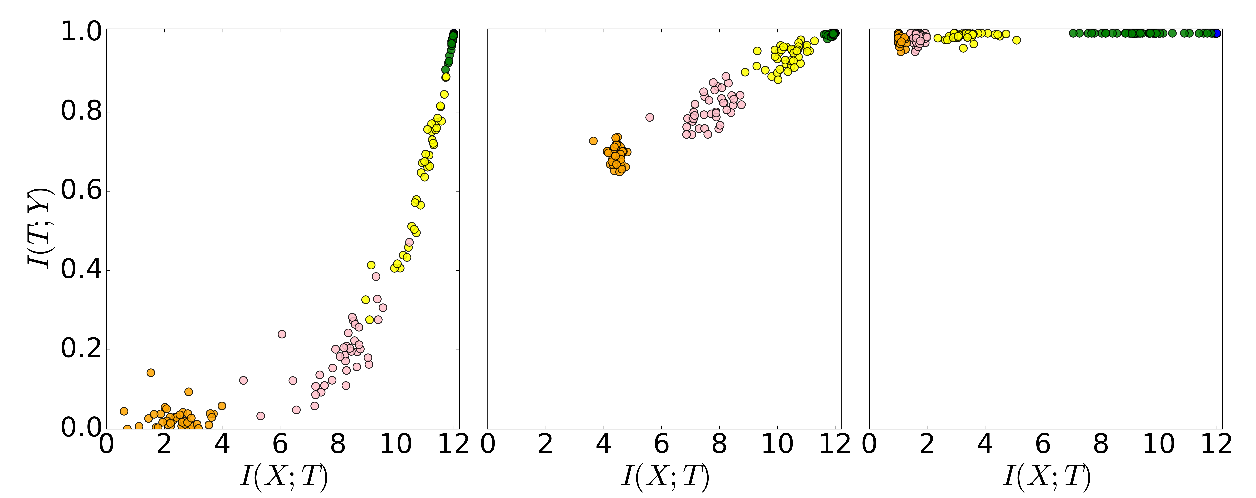
\includegraphics[width=\textwidth]{../presentation/InformationPlane.png}
	\caption{Snapshots of layers of 50 randomized networks: left - with the initial weights; center - at 400 epochs (ERM); right - after 9000 epochs (RC); layers are denoted by color.}
\end{figure}
\paragraph{}
Observation of network's movement on infoplane allowed authors to find out two distinct stages of Stochastic Gradient Descent training:
\subparagraph{ERM}
\begin{itemize}
	\item takes few hundred epochs;
	\item layers increase information on labels;
	\item order of layers is preserved;
\end{itemize}
\subparagraph{Representation compression}
\begin{itemize}
	\item takes a lot of time;
	\item layers drop irrelevant information on input data;
\end{itemize}
\paragraph{}
Authors try to further investigate ERM and representation-compression phases by looking at behavior of of the stochastic gradients along the epochs (figure below\cite{shwartz2017opening}):
\begin{figure}[!h]
	\centering
	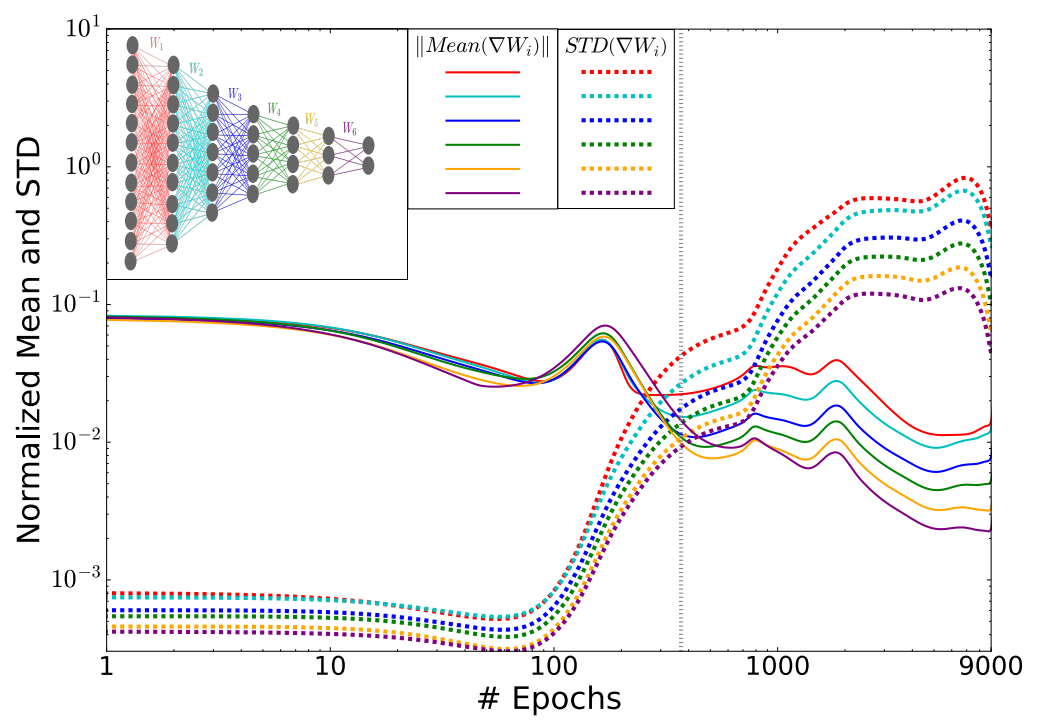
\includegraphics[width=\textwidth]{SGD.png}
	\caption{The layers’ Stochastic Gradients distributions during the optimization process. The norm of the means and standard deviations of the weights gradients for each layer, as function of the number of training epochs (in log-log scale).}
\end{figure}
\paragraph{}
The transition between two phases of SGD is clearly seen on the plot (marked by gray line). The first is a \textit{drift} phase, where the gradient means are much larger than their standard deviations, indicating small gradient stochasticity and in the second phase called the \textit{diffusion} phase, the gradient means are very small compared to their batch to batch fluctuations, and the gradients behave like Gaussian noise with very small means, for each layer.
\paragraph{}
Authors note the very significant consequence of representation compression by diffusion: there are a lot of different networks with optimal performance so any attempt to interpret a weight or an output of neuron is meaningless. Next time the network will not converge to the same optimal set of weights but to different one.

\section{Hidden layers}
To understand why the network needs hidden layers they have conducted a series of experiments (results are shown below\cite{shwartz2017opening}) as follows:
\begin{enumerate}
	\item 6 different architectures with 1 to 6 hidden layers;
	\item Repeat each experiment 50 times with randomized initial weights and training samples.
\end{enumerate}
\paragraph{}
\begin{figure}[!h]
	\centering
	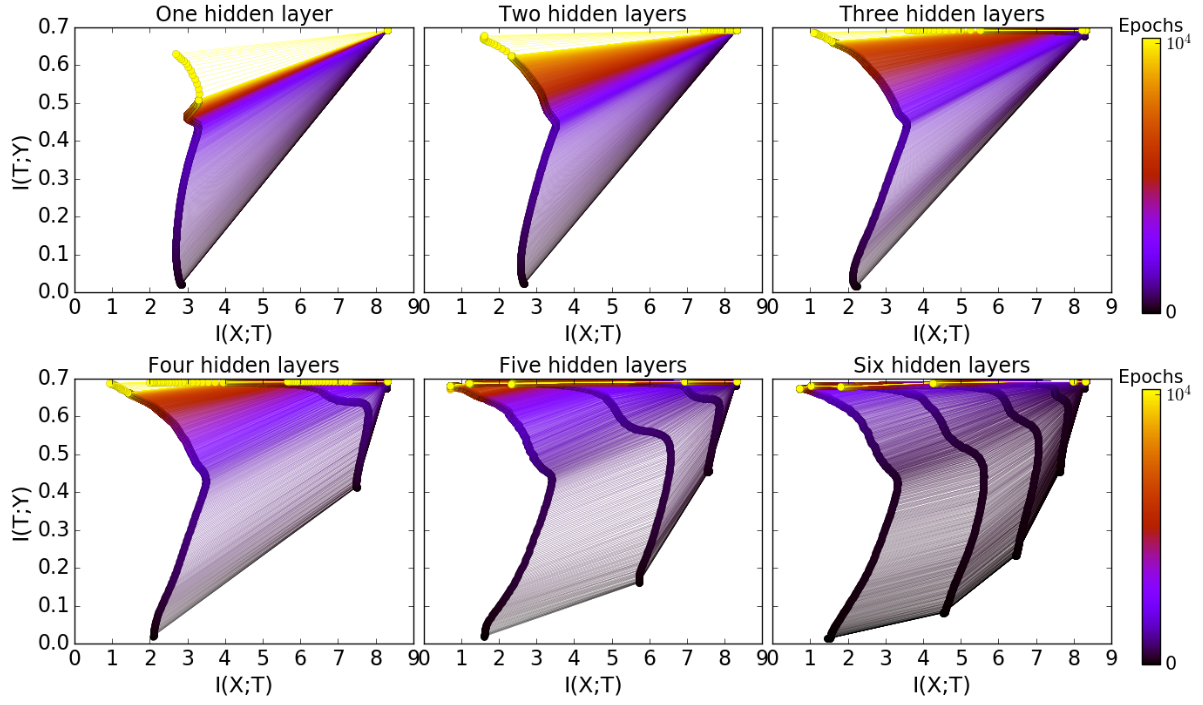
\includegraphics[width=\textwidth]{../presentation/InformationPaths.png}
	\caption{The layers information paths during the SGD optimization for different architectures.
Each panel is the information plane for a network with a different number of
hidden layers. The width of the hidden layers start with 12, and each additional layer has
2 fewer neurons. The final layer with 2 neurons is shown in all panels. The line colors
correspond to the number of training epochs.}
\end{figure}
\paragraph{}
They have reached the following results:
\begin{itemize}
		\item More hidden layers - good generalization is reached faster;
		\item Compression phase of a layer is shorter if it is started from previously compressed layer;
		\item For the deeper layers the compression is faster;
		\item Wide layers also eventually converge in diffusion.
	\end{itemize}
\section{Numerical experiments setup}
\paragraph{}
In this section I describe my experimental setup. I have tried to reproduce some of Schwarz-Ziv and Tishby results on a different setup. The idea is to see whether those results are invariant to:
\begin{itemize}
	\item the task at hand - Schwarz-Ziv and Tishby used a toyish task that was easy to solve and analyze. I've tried more difficult real data task - identification of digits on MNIST\cite{lecun1998mnist};
	\item the way to estimate Mutual Information - Schwarz-Ziv and Tishby used a very direct method that is constructed easily for their toy task (I omit the description of their method here, look for it at \cite{shwartz2017opening}). I use NPEET library\cite{ver2000non} for non-parametric general purpose MI estimation;
	\item training algorithm - they used plain SGD, but I used Adam\cite{kingma2014adam} since it is the most used variation of SGD for now.
\end{itemize}
\paragraph{}
MNIST (Mixed National Institute of Standards and Technology) is a database that contains a lot of hand-written digits. It is a very popular benchmark that allows to compare the performance of different Machine Learning models.
\paragraph{}
Typical MNIST workflow is as follows:
\begin{enumerate}
	\item Split the MNIST into test and train sets;
	\item Train the model using raw pixels as an input and 10 classes as a label;
	\item Test the model on hold-out set;
\end{enumerate}
\paragraph{}
For this report to simplify things I use only 1000 numbers from MNIST as train set and 100 numbers as test set. Also I'll train the models not to classify label of a digit, but to regress an actual digit. As loss function I use mean absolute error:
\begin{equation}
	MAE = \frac{1}{n}\sum_{i}|y_{prediction} - y_{real}|
\end{equation}
\paragraph{}
For this report I am not interested in performance of the models in terms of accuracy or mean absolute error, I only want to reproduce the plots similar to \ref{snapshot}.
\paragraph{}
All code to reproduce my experiments can be obtained from \cite{mygithub}.
\section{Results of numerical experiments}
\paragraph{}
The network used is fully-connected with 4 [256,128,64,32] hidden layers, trained to perform Regression. Activations are ELU everywhere except the output layer which is Linear. The layer is marked by color in the following way: black, red, green, blue, yellow.
\paragraph{}
As you can see below the plot complies with the respective plot of Schwarz-Ziv and Tishby. We see that after 400 and 9000 epochs MI between representation and label went up, the clear order of layers started to emerge (from black(input) to yellow(output)).
\begin{figure}[h!]
	\centering
	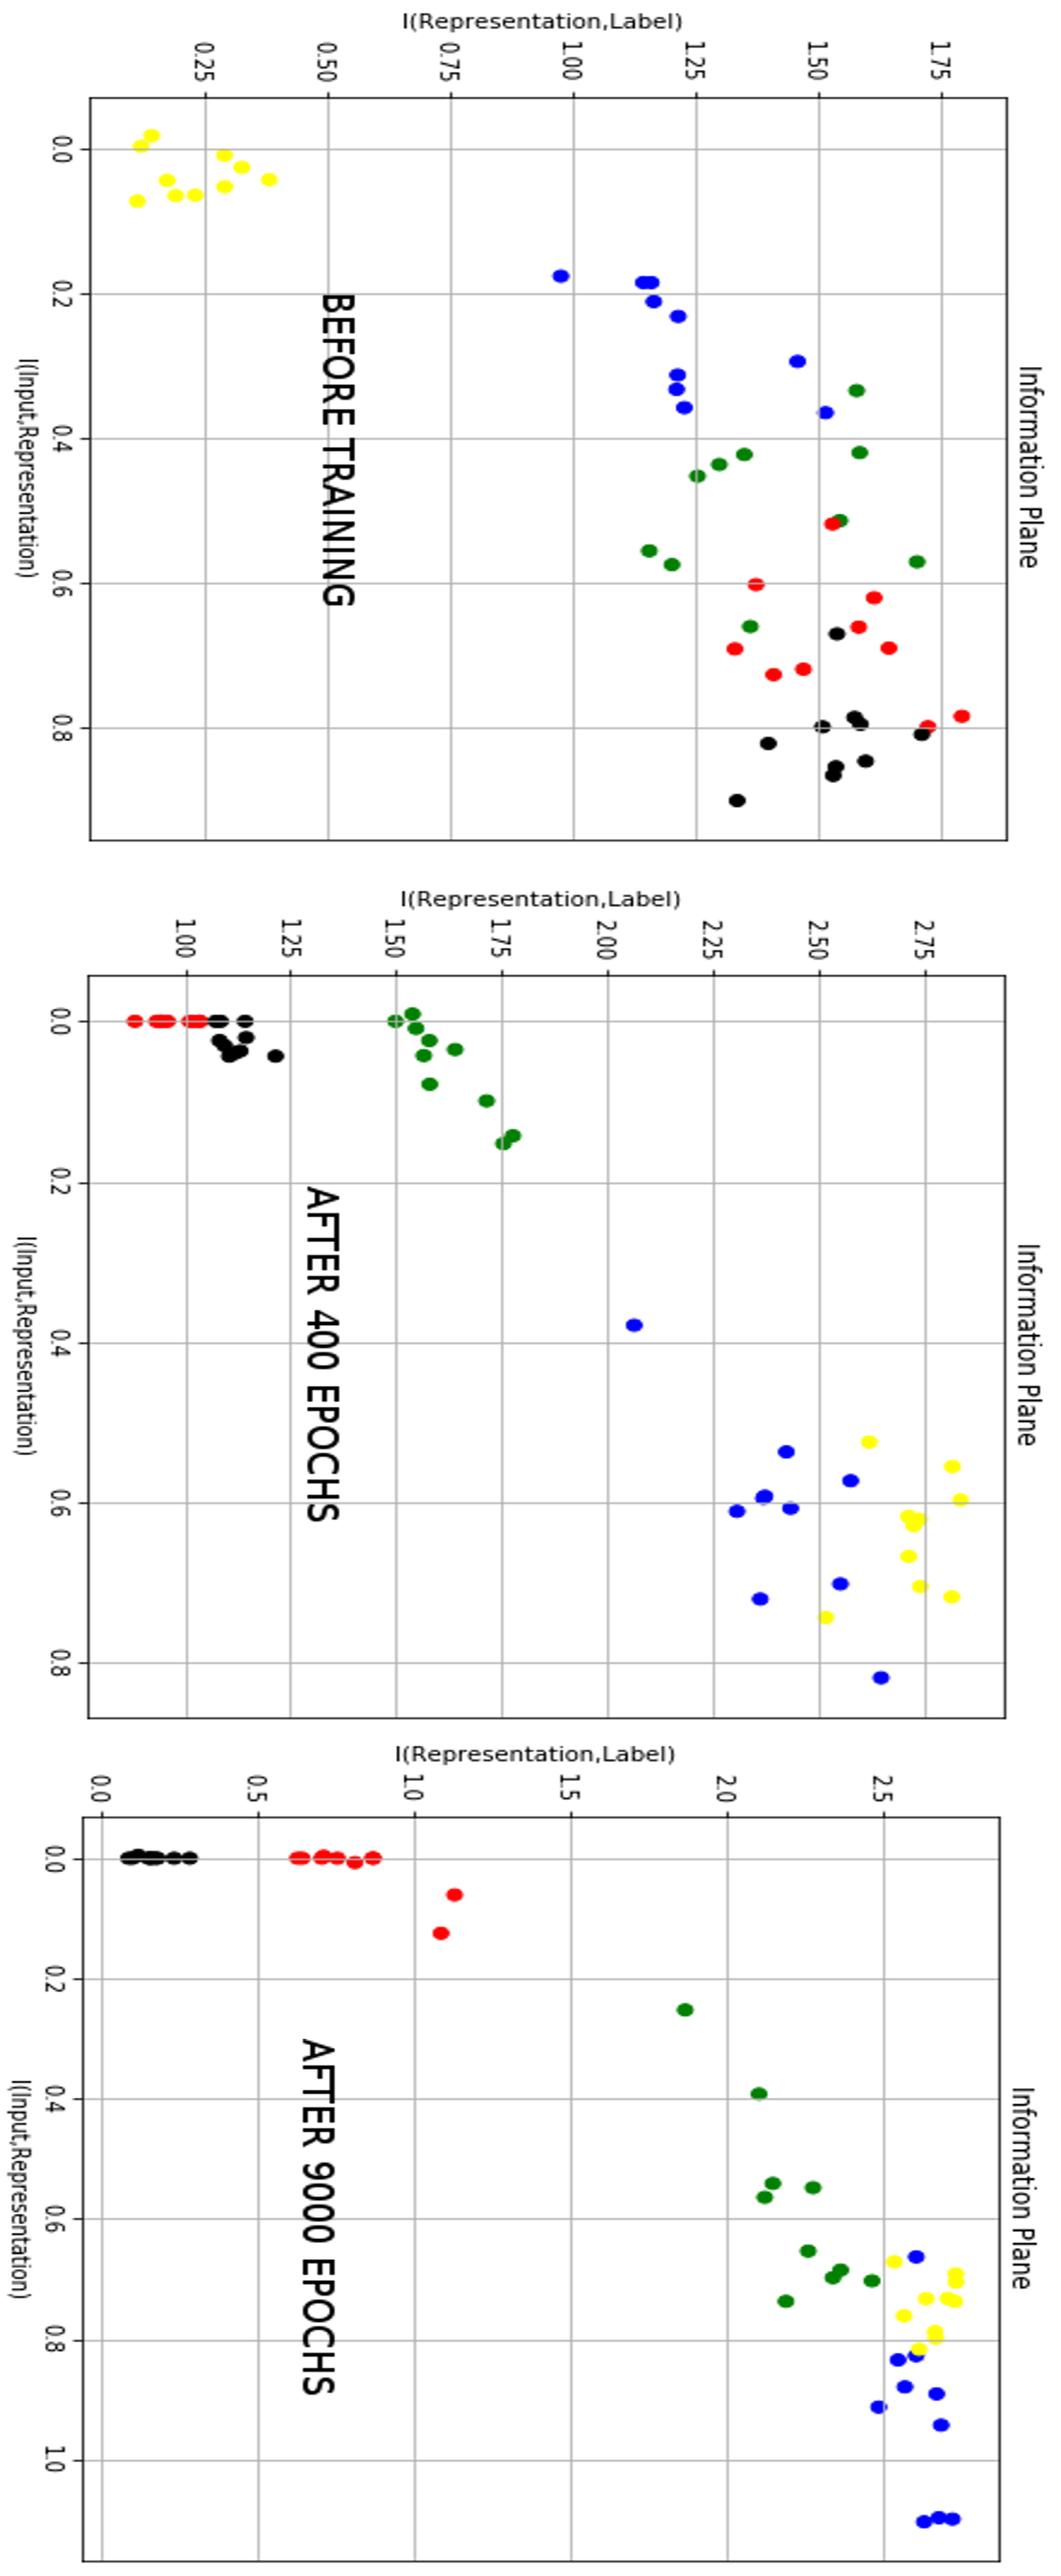
\includegraphics[width=0.55\textwidth]{SnapshotReproduction.png}
	\caption{MNIST Information Plane snapshots}
\end{figure}
\section{Discussion}
\paragraph{}
For me, the one most important thing from this paper is that it is possible to reason about model training in terms of moving around the infoplane. It offers quite a range of possibilities:
\begin{itemize}
	\item Easy visual comparison of the model's performance. If one has two models A and B and A is higher on Y-axis and farther at X-axis from (0,0) than B, one can say that A is better trained because is able to extract more from the data and predicts the label better;
	\item IB tradeoff can be used as a promising loss function. If one wants a good model, one can add the IB tradeoff to existing loss function as a regularization term, or just use the tradeoff instead of typical loss;
	\item Further investigation in this direction can lead to new insight into inner mechanisms of DNNs.
\end{itemize}
\paragraph{}
Schwarz-Ziv and Tishby provide the library called IDNNs \cite{idnns} that can be used to visualize information plane and network behavior.
\paragraph{}
Information Bottleneck as loss function is already implemented in \cite{alemi2016deep}. They parametrize IB as Neural Network, leverage the reparameterization trick for efficient training and got 1.13\% error on MNIST. As a byproduct they have found out that IB loss improves robustness to adversarial inputs. This direction also is worth investigating
\paragraph{}
The other inspiring thing is that they results actually are invariant to changes I descirbed in previous two sections. Scientific result should be the same regardless of method it was obtained by. It implies that IB-approach could be of good use for Deep Learning practitioners in both industry and science.
\newpage
\printbibliography

\end{document}